\documentclass{article}

\usepackage{array}
\usepackage{amsmath}
\usepackage{graphicx}

\begin{document}

\title{Week 6, Session 2 Solutions}
\author{GSI: Caleb Eades}
\date{9/27}
\maketitle

\section{Coulomb's Law}

\subsection{Charges in a Bowl}

\begin{itemize}
	\item[(a)] If the charges are separated by some angle $\theta$, then the physical distance separating them is
	\begin{equation}
	d = 2Rsin\left(\frac{\theta}{2}\right)
	\end{equation}
	From Newton's second law, we garner
	\begin{align*}
	Ncos\frac{\theta}{2} &= mg \\
	Nsin\frac{\theta}{2} &= \frac{1}{4\pi\epsilon_0}\frac{Q^2}{d^2} \\
	&= \frac{1}{4\pi\epsilon_0}\frac{Q^2}{4R^2sin^2\frac{\theta}{2}}
	\end{align*}
	From the first equation, $N = \frac{mg}{cos\frac{\theta}{2}}$. From the second,
	\begin{align*}
	Q^2 &= 16\pi\epsilon_0 R^2 N sin^3\frac{\theta}{2} \\
	&= 16\pi\epsilon_0 mgR^2 tan\frac{\theta}{2}sin^2\frac{\theta}{2} \\
	Q &= 4Rsin\frac{\theta}{2}\sqrt{\pi\epsilon_0 mgtan\frac{\theta}{2}}
	\end{align*}
	\item[(b)] Yes, this is a stable equilibrium since it has a restoring force. Try your hand at solving for the frequency if you want (it is not trivial).
\end{itemize}

\newpage

\subsection{Oh Charge, Where Art Thou?}

We must have
\begin{align*}
\frac{qQ}{4\pi\epsilon_0 d^2} &= \frac{4qQ}{4\pi\epsilon_0 (L-d)^2} \\
\frac{(L-d)^2}{d^2} &= 4 \\
\left(\frac{L}{d}-1\right)^2 &= 4 \\
\frac{L}{d} &= 1\pm 2 \\
L &= 3d,
\end{align*}
where we have chosen the positive answer since $d$ must be between $0$ and $L$. Now, to find $Q$,
\begin{align*}
\frac{4q^2}{4\pi\epsilon_0 L^2} + \frac{4qQ}{4\pi\epsilon_0 (L-d)^2} &= 0 \\
\frac{4q}{L^2} + \frac{4Q}{4L^2/9} &= 0 \\
Q &= - \frac{4}{9}q
\end{align*}

\newpage

\subsection{Return of the Spring}

\begin{itemize}
	\item[(a)] The net force on each charge must be zero:
	\begin{equation}
	\frac{Q^2}{4\pi\epsilon_0 D^2} = k_s (D-L)
	\end{equation}
	\item[(b)] Same as part (a) since like charges repel, regardless of whether the like charges are both positive or both negative.
	\item[(c)] If they have opposite signs but the same magnitude, $Q = |Q_1| = |Q_2|$ and
	\begin{equation}
	\frac{Q^2}{4\pi\epsilon_0 D^2} = k_s (L-D)
	\end{equation}
\end{itemize}

\newpage

\subsection{A Balancing Act}

\begin{itemize}
	\item[(a)] We must have
	\begin{align*}
	\frac{qQ}{4\pi\epsilon_0 d^2} &= mg \\
	d &= \sqrt{\frac{qQ}{4\pi\epsilon_0 mg}}
	\end{align*}
	\item[(b)] No, this is not a stable equilibrium. If we go a little higher, the charges will attract stronger than gravity and it will keep rising. If we go a little lower, the gravitational pull will be stronger than the electric forces and it will keep falling.
\end{itemize}

\newpage

\subsection{Dipoles}

Consider the following picture (apologies for the terrible drawing, I'm new to linux and haven't found a great tool yet):
\begin{figure}[h]
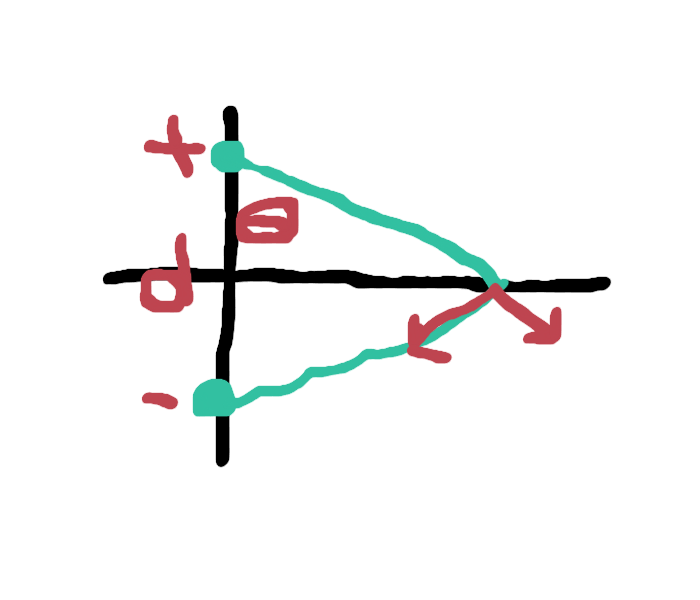
\includegraphics[width=0.5\textwidth]{dipole.png}
\end{figure}
Hence, the electric field components in the x direction cancel and we are left with a field solely in the negative y direction. That is,
\begin{align*}
\vec{E} &= \vec{E_{+}} + \vec{E_{-}} \\
&= -2\frac{q}{4\pi\epsilon_0 r^2}cos\theta \hat{y} \\
&= \frac{-qd}{4\pi\epsilon_0 r^3}\hat{y} \\
&= \frac{-p}{4\pi\epsilon_0 r^3}\hat{y}
\end{align*}
where $p=qd$ is the dipole moment. Taking the limit as $d\rightarrow 0$ while $p$ remains constant, the field from a pure dipole in the plane perpendicular to the moment is given by
\begin{equation}
\vec{E} = \frac{-\vec{p}}{4\pi\epsilon_0 r^3}
\end{equation}
Note that $r$ here is really from one of the charges to the point in the perpendicular plane, but since we took the limit $d\rightarrow 0$, it is just the distance from the pure dipole (of zero length at the origin) to the point of interest in the perpendicular plane.

Now, along the axis of the dipole moment,
\begin{align*}
\vec{E} &= \left(\frac{q}{4\pi\epsilon_0 (r-d/2)^2}-\frac{q}{4\pi\epsilon_0 (r+d/2)^2}\right)\hat{y} \\
&= kq\left[(r-d/2)^{-2} - (r+d/2)^{-2}\right]\hat{y}
\end{align*}
Again taking the limit as $d\rightarrow 0$ while $p$ remains constant, we will use the Binomial approximation:
\begin{align*}
\vec{E} &= \frac{kq}{r^2}\left[(1-d/2r)^{-2} - (1+d/2r)^{-2}\right]\hat{y} \\
&= \frac{kq}{r^2}\left[1+d/r-1+d/r\right]\hat{y} \\
&= \frac{2k\vec{p}}{r^3}
\end{align*}
Hence, the field from a pure dipole along the dipole moment is given by
\begin{equation}
\vec{E} = \frac{\vec{p}}{2\pi\epsilon_0 r^3}
\end{equation}

\end{document}
